\documentclass[a4paper, 12pt]{article}
\usepackage{amsmath}
\usepackage{amssymb}
\usepackage[left=2cm, right=2cm, bottom=3cm, top=2cm]{geometry}
\usepackage{graphicx}
\usepackage[utf8]{inputenc}
\usepackage{microtype}
\usepackage{natbib}

\newcommand{\Cauchy}{\textnormal{Cauchy}}
\newcommand{\Celery}{{\em Celery}}
\newcommand{\Exponential}{\textnormal{Exponential}}
\newcommand{\given}{\,|\,}
\newcommand{\Laplace}{\textnormal{Laplace}}
\newcommand{\location}{\textnormal{location}}
\newcommand{\Normal}{\textnormal{Normal}}
\newcommand{\scale}{\textnormal{scale}}
\newcommand{\Uniform}{\textnormal{Uniform}}


\title{The~\Celery~ model specification}
%\author{Brendon J. Brewer}
\date{}

\begin{document}
\maketitle

%\abstract{\noindent Abstract}

% Need this after the abstract
\setlength{\parindent}{0pt}
\setlength{\parskip}{1em}

Let $\boldsymbol{y} = \{y_1, y_2, ..., y_n\}$ be the vector of measurements
taken at times $\boldsymbol{t} = \{t_1, t_2, ..., t_n\}$. Assume that the
observers have provided ``error bars''
$\boldsymbol{\sigma} = \{\sigma_1, \sigma_2, ..., \sigma_n\}$ along with the
measurements.

\section{Parameters and Hyperparameters}

\subsection{Oscillation parameters and hyperparameters}

Let the unknown parameters be $M$, the number of oscillation modes,
$\boldsymbol{T} = \{T_1, T_2, ..., T_M\}$ their periods,
$\boldsymbol{A} = \{A_1, A_2, ..., A_M\}$ their amplitudes,
and $\boldsymbol{Q} = \{Q_1, Q_2, ..., Q_M\}$ their qualities.

The prior for the number of modes $M$ is
\begin{align}
p(M) &\propto \frac{1}{M}
\end{align}
for $M \in \{0, 1, 2, ..., M_{\rm max}\}$. By default, the maximum number of
modes is $M_{\rm max} = 30$.

The priors for these are
\begin{align}
\ln T_i &\sim \Laplace(\location=a_T, \scale=b_T) \\
A_i &\sim \Exponential(\scale=\mu_A) \\
\ln Q_i &\sim \Laplace(\location=a_Q, \scale=b_Q)
\end{align}
where some hyperparameters relating to periods, amplitudes, and qualities
have been introduced. The priors for these hyperparameters are:
\begin{align}
\ln a_T   &\sim \Uniform(10^{-6}t_{\rm range}, t_{\rm range}) \\
\ln b_T   &\sim \Uniform(0, 2)\\
\ln \mu_A &\sim \Cauchy(\location=0, \scale=5)T(-50, 50) \\
\ln a_Q   &\sim \Uniform(0, \ln (1000)) \\
\ln b_Q   &\sim \Uniform(0, 1)
\end{align}
The notation $T(,)$ denotes truncation, as in the BUGS language.

\subsection{``Extra noise'' parameters}

The error bars provided by the observers may or may not be trustworthy, and
there also might be correlated noise (or non-oscillatory signal) in the data.
The correlated noise is assumed to have a mean parameter of zero
and an exponential covariance function
\begin{align}
C_{\rm extra}(\tau) &= A_{\rm extra}\exp\left(-|\tau| / L\right)
\label{eqn:red_noise}
\end{align}
where $\tau$ is the time separation, and $A_{\rm extra}$, $L$ are
hyperparameters. The priors for the hyperparameters are
\begin{align}
\ln A_{\rm extra} &\sim \Normal(\location=\mu_A, \scale=10) \\
\ln L &\sim \Normal(\location=t_{\rm range}, \scale=10)
\end{align}

The given error bars are considered to be trustworthy with prior probability
0.5. If not, they are enlarged by some factor greater than one. Let $k$ be
the factor by which the error bars are inflated. The prior for $k$ is
\begin{align}
p(k) &= \frac{1}{2}\delta(k-1) + \frac{1}{2}\frac{1}{x^2}
\end{align}
for $k \geq 1$. This is a 50/50 mixture of a delta function at $k=1$
and a Pareto distribution with a shape parameter of 1.

\section{Justifications for the choices of priors}

Rough justifications for these choices are as follows:
\begin{itemize}
    \item The amplitudes, all positive, will be scattered around some typical
          value, but we don't know it. The data is likely to be supplied
          in units where amplitudes are probably
          within a few orders of magnitude of unity.
    \item The periods, all positive, will be scattered around some typical
          value we don't know, but the typical period is probably shorter
          (and possibly much shorter) than the time-range of the measurements.
          Periods probably don't vary by much more than an order of magnitude.
    \item The qualities, all positive, will be scattered around some typical
          value that is probably of order tens to hundreds. The mode qualities
          are unlikely to differ from each other by a large margin.
    \item The number of modes is unknown, but for pragmatic computational
          reasons we weakly favour smaller numbers of modes (the prior
          is approximately a discrete log-uniform).
    \item The amplitude of the extra red noise is likely to be within
          several orders of magnitude of the amplitude of the oscillations.
    \item The characteristic timescale of the extra red noise is likely to
          be within several orders of magnitude of the time range of the
          observations.
    \item The error bar inflation parameter could be 1, or it could be
          greater than 1 but probably not my many orders of magnitude.
\end{itemize}

\section{Conditional prior for the measurements}

The probability distribution for the measurements given the parameters is
a gaussian process with mean function of zero and covariance matrix given
by the sum of $M$ quasiperiodic terms (one for each mode, each of which
has the form as Equation 23 of \citet{celerite}), plus the red noise
(Equation~\ref{eqn:red_noise}), plus $k\boldsymbol{\sigma}$ on the diagonal.

\section{PGM}

\begin{figure}[!ht]
\centering
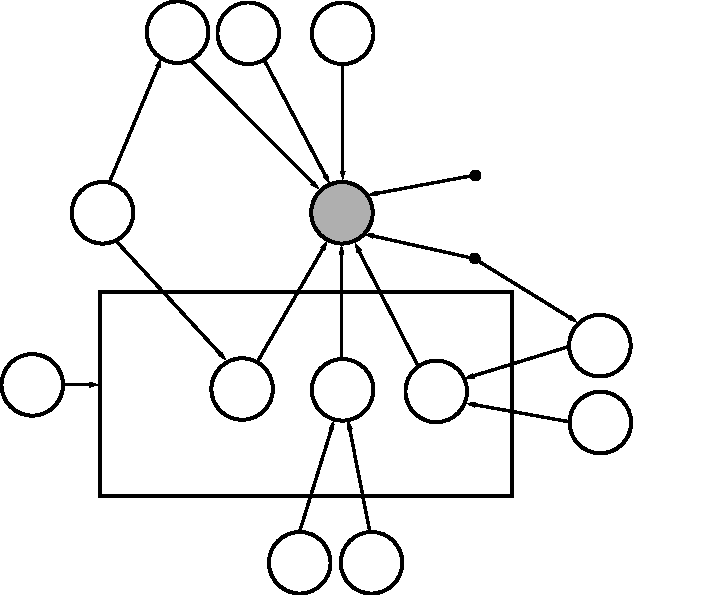
\includegraphics{pgm.pdf}
\caption{\label{fig:pgm}}
\end{figure}

\begin{thebibliography}{999}
\bibitem[Foreman-Mackey et al.(2017)]{celerite}
Foreman-Mackey, D., Agol, E., Ambikasaran, S. and Angus, R., 2017. Fast and scalable Gaussian process modeling with applications to astronomical time series. The Astronomical Journal, 154(6), p.220.
\end{thebibliography}

\end{document}

